\documentclass[]{book}
\usepackage{lmodern}
\usepackage{amssymb,amsmath}
\usepackage{ifxetex,ifluatex}
\usepackage{fixltx2e} % provides \textsubscript
\ifnum 0\ifxetex 1\fi\ifluatex 1\fi=0 % if pdftex
  \usepackage[T1]{fontenc}
  \usepackage[utf8]{inputenc}
\else % if luatex or xelatex
  \ifxetex
    \usepackage{mathspec}
  \else
    \usepackage{fontspec}
  \fi
  \defaultfontfeatures{Ligatures=TeX,Scale=MatchLowercase}
\fi
% use upquote if available, for straight quotes in verbatim environments
\IfFileExists{upquote.sty}{\usepackage{upquote}}{}
% use microtype if available
\IfFileExists{microtype.sty}{%
\usepackage{microtype}
\UseMicrotypeSet[protrusion]{basicmath} % disable protrusion for tt fonts
}{}
\usepackage{hyperref}
\hypersetup{unicode=true,
            pdftitle={A Tidy Introduction To Statistical Learning},
            pdfauthor={Beau Lucas},
            pdfborder={0 0 0},
            breaklinks=true}
\urlstyle{same}  % don't use monospace font for urls
\usepackage{natbib}
\bibliographystyle{apalike}
\usepackage{color}
\usepackage{fancyvrb}
\newcommand{\VerbBar}{|}
\newcommand{\VERB}{\Verb[commandchars=\\\{\}]}
\DefineVerbatimEnvironment{Highlighting}{Verbatim}{commandchars=\\\{\}}
% Add ',fontsize=\small' for more characters per line
\usepackage{framed}
\definecolor{shadecolor}{RGB}{248,248,248}
\newenvironment{Shaded}{\begin{snugshade}}{\end{snugshade}}
\newcommand{\AlertTok}[1]{\textcolor[rgb]{0.94,0.16,0.16}{#1}}
\newcommand{\AnnotationTok}[1]{\textcolor[rgb]{0.56,0.35,0.01}{\textbf{\textit{#1}}}}
\newcommand{\AttributeTok}[1]{\textcolor[rgb]{0.77,0.63,0.00}{#1}}
\newcommand{\BaseNTok}[1]{\textcolor[rgb]{0.00,0.00,0.81}{#1}}
\newcommand{\BuiltInTok}[1]{#1}
\newcommand{\CharTok}[1]{\textcolor[rgb]{0.31,0.60,0.02}{#1}}
\newcommand{\CommentTok}[1]{\textcolor[rgb]{0.56,0.35,0.01}{\textit{#1}}}
\newcommand{\CommentVarTok}[1]{\textcolor[rgb]{0.56,0.35,0.01}{\textbf{\textit{#1}}}}
\newcommand{\ConstantTok}[1]{\textcolor[rgb]{0.00,0.00,0.00}{#1}}
\newcommand{\ControlFlowTok}[1]{\textcolor[rgb]{0.13,0.29,0.53}{\textbf{#1}}}
\newcommand{\DataTypeTok}[1]{\textcolor[rgb]{0.13,0.29,0.53}{#1}}
\newcommand{\DecValTok}[1]{\textcolor[rgb]{0.00,0.00,0.81}{#1}}
\newcommand{\DocumentationTok}[1]{\textcolor[rgb]{0.56,0.35,0.01}{\textbf{\textit{#1}}}}
\newcommand{\ErrorTok}[1]{\textcolor[rgb]{0.64,0.00,0.00}{\textbf{#1}}}
\newcommand{\ExtensionTok}[1]{#1}
\newcommand{\FloatTok}[1]{\textcolor[rgb]{0.00,0.00,0.81}{#1}}
\newcommand{\FunctionTok}[1]{\textcolor[rgb]{0.00,0.00,0.00}{#1}}
\newcommand{\ImportTok}[1]{#1}
\newcommand{\InformationTok}[1]{\textcolor[rgb]{0.56,0.35,0.01}{\textbf{\textit{#1}}}}
\newcommand{\KeywordTok}[1]{\textcolor[rgb]{0.13,0.29,0.53}{\textbf{#1}}}
\newcommand{\NormalTok}[1]{#1}
\newcommand{\OperatorTok}[1]{\textcolor[rgb]{0.81,0.36,0.00}{\textbf{#1}}}
\newcommand{\OtherTok}[1]{\textcolor[rgb]{0.56,0.35,0.01}{#1}}
\newcommand{\PreprocessorTok}[1]{\textcolor[rgb]{0.56,0.35,0.01}{\textit{#1}}}
\newcommand{\RegionMarkerTok}[1]{#1}
\newcommand{\SpecialCharTok}[1]{\textcolor[rgb]{0.00,0.00,0.00}{#1}}
\newcommand{\SpecialStringTok}[1]{\textcolor[rgb]{0.31,0.60,0.02}{#1}}
\newcommand{\StringTok}[1]{\textcolor[rgb]{0.31,0.60,0.02}{#1}}
\newcommand{\VariableTok}[1]{\textcolor[rgb]{0.00,0.00,0.00}{#1}}
\newcommand{\VerbatimStringTok}[1]{\textcolor[rgb]{0.31,0.60,0.02}{#1}}
\newcommand{\WarningTok}[1]{\textcolor[rgb]{0.56,0.35,0.01}{\textbf{\textit{#1}}}}
\usepackage{longtable,booktabs}
\usepackage{graphicx,grffile}
\makeatletter
\def\maxwidth{\ifdim\Gin@nat@width>\linewidth\linewidth\else\Gin@nat@width\fi}
\def\maxheight{\ifdim\Gin@nat@height>\textheight\textheight\else\Gin@nat@height\fi}
\makeatother
% Scale images if necessary, so that they will not overflow the page
% margins by default, and it is still possible to overwrite the defaults
% using explicit options in \includegraphics[width, height, ...]{}
\setkeys{Gin}{width=\maxwidth,height=\maxheight,keepaspectratio}
\IfFileExists{parskip.sty}{%
\usepackage{parskip}
}{% else
\setlength{\parindent}{0pt}
\setlength{\parskip}{6pt plus 2pt minus 1pt}
}
\setlength{\emergencystretch}{3em}  % prevent overfull lines
\providecommand{\tightlist}{%
  \setlength{\itemsep}{0pt}\setlength{\parskip}{0pt}}
\setcounter{secnumdepth}{5}
% Redefines (sub)paragraphs to behave more like sections
\ifx\paragraph\undefined\else
\let\oldparagraph\paragraph
\renewcommand{\paragraph}[1]{\oldparagraph{#1}\mbox{}}
\fi
\ifx\subparagraph\undefined\else
\let\oldsubparagraph\subparagraph
\renewcommand{\subparagraph}[1]{\oldsubparagraph{#1}\mbox{}}
\fi

%%% Use protect on footnotes to avoid problems with footnotes in titles
\let\rmarkdownfootnote\footnote%
\def\footnote{\protect\rmarkdownfootnote}

%%% Change title format to be more compact
\usepackage{titling}

% Create subtitle command for use in maketitle
\providecommand{\subtitle}[1]{
  \posttitle{
    \begin{center}\large#1\end{center}
    }
}

\setlength{\droptitle}{-2em}

  \title{A Tidy Introduction To Statistical Learning}
    \pretitle{\vspace{\droptitle}\centering\huge}
  \posttitle{\par}
    \author{Beau Lucas}
    \preauthor{\centering\large\emph}
  \postauthor{\par}
      \predate{\centering\large\emph}
  \postdate{\par}
    \date{2019-08-06}

\usepackage{booktabs}
\usepackage{amsthm}
\makeatletter
\def\thm@space@setup{%
  \thm@preskip=8pt plus 2pt minus 4pt
  \thm@postskip=\thm@preskip
}
\makeatother

\begin{document}
\maketitle

{
\setcounter{tocdepth}{1}
\tableofcontents
}
\hypertarget{preface}{%
\chapter*{Preface}\label{preface}}
\addcontentsline{toc}{chapter}{Preface}

This book will serve as a source of notes and exercise solutions for \emph{An Introduction to Statistical Learning}. My approach will be centered around the \texttt{tidyverse}. This is not a replacement for the book, which should be read front to back by all machine learning enthusiasts.

Chapter names will line up, and certain subheadings will also match. Sometimes my notes will contain text lifted straight from the book without modification. This is not an attempt to plagiarize or claim their writing as my own. My goal is for this bookdown project to be a quick stop for machine learning enthusiasts to reference high-level ideas from ISLR in a modern media format.

\hypertarget{intro}{%
\chapter{Introduction}\label{intro}}

\begin{center}\rule{0.5\linewidth}{\linethickness}\end{center}

\hypertarget{an-overview-of-statistical-learning}{%
\section{An Overview of Statistical Learning}\label{an-overview-of-statistical-learning}}

Statistical learning is focused on supervised and unsupervised modeling and prediction.

\hypertarget{data-sets-used-in-labs-and-exercises}{%
\section{Data Sets Used in Labs and Exercises}\label{data-sets-used-in-labs-and-exercises}}

All data sets used in this book can be found in \texttt{ISLR} and \texttt{MASS} packages, with some also being found in the base \texttt{R} distribution.

We will utilize the \texttt{tidyverse} ecosystem to tackle the exercises and labs, as the \texttt{R} code found in the original textbook is outdated.

\begin{Shaded}
\begin{Highlighting}[]
\KeywordTok{require}\NormalTok{(ISLR)}
\KeywordTok{require}\NormalTok{(MASS)}
\KeywordTok{require}\NormalTok{(tidyverse)}
\KeywordTok{require}\NormalTok{(knitr)}
\KeywordTok{require}\NormalTok{(kableExtra)}
\KeywordTok{require}\NormalTok{(modelr)}
\end{Highlighting}
\end{Shaded}

\hypertarget{book-website}{%
\section{Book Website}\label{book-website}}

The website and free PDF for the book can be found here:

\href{http://www-bcf.usc.edu/~gareth/ISL/}{www.statlearning.com}

And here are the YouTube lectures an R labs:

\href{https://www.youtube.com/channel/UC4OWDcPB1peiBXDfCSZ3h-w}{Youtube - Statistical Learning}

\hypertarget{statistical-learning}{%
\chapter{Statistical Learning}\label{statistical-learning}}

\begin{center}\rule{0.5\linewidth}{\linethickness}\end{center}

\hypertarget{what-is-statistical-learning}{%
\section{What is Statistical Learning?}\label{what-is-statistical-learning}}

Methods to estimate functions that connect inputs to outputs.

If there exists a quantitative response variable \(Y\) and \(p\) different predictors (\(X_1\), \(X_2\), \ldots{}, \(X_p\)), we can write this relationship as:

\(Y = f(X) + ε\)

\hypertarget{why-estimate-f}{%
\subsection{\texorpdfstring{Why Estimate \emph{\(f\)}?}{Why Estimate f?}}\label{why-estimate-f}}

\hypertarget{prediction}{%
\subsubsection{Prediction}\label{prediction}}

We can predict Y using:

\(\hat{Y} = \hat{f}(X)\)

Accuracy of \(Y\) is dependant on:

\begin{itemize}
\tightlist
\item
  \emph{reducible error}

  \begin{itemize}
  \tightlist
  \item
    \(\hat{f}\) will never be perfect estimate of \(f\), and model can always be potentially improved
  \item
    Even if \(\hat{f} = f\), prediction would still have some error
  \end{itemize}
\item
  \emph{irreducible error}

  \begin{itemize}
  \tightlist
  \item
    Because \(Y\) is also a function of random \(ε\), there will always be variability
  \item
    We cannot reduce the error introduced by \(ε\)
  \end{itemize}
\end{itemize}

\hypertarget{inference}{%
\subsubsection{Inference}\label{inference}}

How does \(Y\) respond to changes in \(X_1, X_2, ..., X_p\)?

\hypertarget{how-do-we-estimate-f}{%
\subsection{\texorpdfstring{How do we estimate \emph{\(f\)}?}{How do we estimate f?}}\label{how-do-we-estimate-f}}

\begin{itemize}
\tightlist
\item
  Use \emph{training data} to train method
\item
  \(x_ij\) is value of \(j\)th predictor for observation \(i\), \(y_i\) is value of response variable

  \begin{itemize}
  \tightlist
  \item
    \(i = 1, 2, ..., n\), \(j = 1, 2, ..., p\)
  \end{itemize}
\item
  Using training data, apply statistical learning method estimate unknown function \(f\)
\item
  Most statistical learning methods can be characterized as either \emph{parametric} or \emph{non-parametric}
\end{itemize}

\hypertarget{parametric-methods}{%
\subsubsection{Parametric Methods}\label{parametric-methods}}

Two-step model-based approach:

\begin{enumerate}
\def\labelenumi{\arabic{enumi}.}
\tightlist
\item
  Make an assumption about functional form of \(f\), such as ``\(f\) is linear in \(X\)''
\item
  Perform procedure that uses training data to train the model
  * In case of linear model, this procedure estimates parameters \(β_0, β_1, ..., β_p\)
  * Most common approach to fit linear model is \emph{(ordinary) least squares}
\end{enumerate}

This is \emph{parametric}, as it reduces the problem of estimating \(f\) down to one of estimating a set of parameters. Problems that can arise:

\begin{itemize}
\tightlist
\item
  Model will not match the true unknown form of \(f\)
\item
  If model is made more \emph{flexible}, which generally requires estimating a greater number of parameters, \emph{overfitting} can occur
\end{itemize}

\hypertarget{non-parametric-methods}{%
\subsubsection{Non-parametric Methods}\label{non-parametric-methods}}

Non-parametric methods do not make assumptions about the form of \(f\). An advantage of this is that they have the potential to fit a wider range of possible shapes for \(f\). A disadvantage is that, because there are no assumptions about the form of \(f\), the problem of estimating \(f\) is not reduced to a set number of parameters. This means more observations are needed compared to a parametric approach to estimate \(f\) accurately.

\hypertarget{the-trade-off-between-prediction-accuracy-and-model-interpretability}{%
\subsection{The Trade-Off Between Prediction Accuracy and Model Interpretability}\label{the-trade-off-between-prediction-accuracy-and-model-interpretability}}

Restrictive models are much more intepretable than flexible ones. Flexible approaches can be so complicated that it is hard to understand how predictors affect the response.

If inference is the goal, simple and inflexible methods are easier to interpret. For prediction, accuracy is the biggest concern. However, flexible models are more prone to overfitting.

\hypertarget{supervised-versus-unsupervised-learning}{%
\subsection{Supervised Versus Unsupervised Learning}\label{supervised-versus-unsupervised-learning}}

Most machine learning methods can be split into \emph{supervised} or \emph{unsupervised} categories. Most of this textbook involves supervised learning methods, in which a model that captures the relationship between predictors and response measurements is fitted. The goal is to accurately predict the response variables for future observations, or to understand the relationship between the predictors and response.

Unsupervised learning takes place when we have a set of observations and a vector of measurements \(x_i\), but no response \(y_i\). We can examine the relationship between the variables or between the observations. A popular method of unsupervised learning is \href{https://en.wikipedia.org/wiki/Cluster_analysis}{cluster analysis}, in which observations are grouped into distinct groups based on their vector of measurements \(x_i\). An example of this would be a company segmenting survey respondents based on demographic data, in which the goal is to ascertain some idea about potential spending habits without possessing this data.

Clustering has some drawbacks. It works best when the groups are significantly distinct from each other. In reality, it is rare for data to exhibit this characteristic. There is often overlap between observations in different groups, and clustering will inevitably place a number of observations in the wrong groups. Further more, visualization of clusters breaks down as the dimensionality of data increases. Most data contains at least several, if not dozens, of variables.

It is not always clear-cut whether a problem should be handled with supervised or unsupervised learning. There are some scenarios where only a subset of the observations have response measurements. This is a \emph{semi-supervised learning} problem, in which a statistical learning method that can utilize all observations is needed.

\hypertarget{regression-versus-classification-problems}{%
\subsection{Regression Versus Classification Problems}\label{regression-versus-classification-problems}}

Variables can be categorized as either \emph{quantitative} or \emph{qualitative}. Both qualitative and quantatitive predictors can be used to predict both types of response variables. The more important part of choosing an appropriate statistical learning method is the type of the response variable.

\begin{center}\rule{0.5\linewidth}{\linethickness}\end{center}

\hypertarget{assessing-model-accuracy}{%
\section{Assessing Model Accuracy}\label{assessing-model-accuracy}}

Every data set is different and there is no one statistical learning method that works best for all data sets. It is important for any given data set to find the statistical learning method that produces the best results. This section presents some concepts that are part of that decision-making process.

\hypertarget{measuring-the-quality-of-fit}{%
\subsection{Measuring the Quality of Fit}\label{measuring-the-quality-of-fit}}

We need to be able to quantify how well a model's predictions match the observed data. How close are the model's predicted response values to the true response values?

In regression, \href{https://en.wikipedia.org/wiki/Mean_squared_error}{\emph{mean squared error (MSE)}} is the most commonly-used measure. A small MSE indicates the predicted responses are very close to the true ones. MSE used on training data is more accurately referred to as the \emph{training MSE}.

We are most concerned with the accuracy of the predictions when we apply our methods to \textbf{previously unseen data}. If you are trying to predict the value of a stock, your concern is how it performs in the future, not on known data from the past. Thus, the goal is then minimizing the \emph{test MSE}, which measures the accuracy of a model on \textbf{observations that were not used to train the model}. Imagine a set of observations \((x_0, y_0)\) that were not used to train the statistical learning method.

\(Ave(y_0 - \hat{f}(x_0))2\)

The goal is to select the model that minimizes the test MSE shown above. How can we do this?

Sometimes, there is an available test data set full of observations that were not used in training the model. The test MSE can be evaluated on these observations, and the learning method which produces the smallest TSE will be chosen. If no test observations are available, picking the method that minimizes the training MSE might seem to be a good idea. However, there is no guarantee that a model with the lowest training MSE also has the lowest test MSE. Models often work in minimizing the training MSE, and can end up with large test MSE.

There is a tradeoff in model flexibility, training MSE, and test MSE. A model that is too flexible can closely match the training data, but perform poorly on the test data. There is a sweet spot to find between model flexibility, training MSE, and test MSE that varies for each unique data set.

\emph{Degrees of freedom} is a quantity that summarizes the flexibility of a curve, discused more fully in Chapter 7. The more inflexible a model is, the fewer degrees of freedom.

As model flexibility increases, training MSE will inevitably decrease, but test MSE may plateau or even rise. A model with a small training MSE and large test MSE is \emph{overfitting the data}, picking up patterns on the training data that don't exist in the test data. Since we expect the training MSE to almost always be lower than the test MSE, overfitting is a specific case when there exists a less flexible model with a smaller test MSE.

\hypertarget{the-bias-variance-trade-off}{%
\subsection{The Bias-Variance Trade-Off}\label{the-bias-variance-trade-off}}

The expected test MSE can be broken down into the sum of three quantities:

\begin{enumerate}
\def\labelenumi{\arabic{enumi}.}
\tightlist
\item
  the \emph{variance} of \(\hat{f}(x_0)\)
\item
  the squared \emph{bias} of \(\hat{f}(x_0)\)
\item
  the variance of the error terms ε
\end{enumerate}

\(E(y_0 - \hat{f}(x_0)^2 = Var(\hat{f}(x_0)) + [Bias(\hat{f}(x_0))]^2+Var(ε)\)

The formula above defines the \emph{expected test MSE}, which can be thought of the average test MSE that would be obtained if we repeatedly estimated \(f\) and tested each at \(x_0\). To minimize expected test MSE, we need to choose a statistical learning method that achieves both low variance and low bias. Since variance and squared bias are nonnegative, the expected test MSE can never be lower than \(Var(ε)\), the irreducible error.

\emph{Variance} refers to how much \(\hat{f}\) would change if repeatedly estimated with different training data sets. Methods with high variance can produce large changes in \(\hat{f}\) through small changes in the training data. Generally, the more flexible a model it is, the higher the variance. Following the observations so closely can cause changes in just a single observation of the training data to result in significant changes to \(\hat{f}\). More inflexible models, such as linear regression, are less susceptible to the effects of changing a single observation.

\emph{Bias} is the error introduced from approximating a complicated problem by a much simpler model. Fitting a linear regression to data that is not linear will always lead to high bias, no matter how many observations are in the training set. More flexible models tend to result in less bias.

More flexible methods lead to higher variance and lower bias. The rate of change between the quantities determines at which point the test MSE is minimized. Bias tends to decrease at a faster rate in the beginning, causing the test MSE to decline. However, when flexibility reaches a certain point, variance will begin to increase faster than bias is decreasing, causing test MSE to rise.

This relationship between bias, variance, and test MSE is known as the \emph{bias-variance tradeoff}. Here is a good article on it: \href{http://scott.fortmann-roe.com/docs/BiasVariance.html}{Understanding the Bias-Variance Tradeoff}

In real-life scenarios where \(f\) is unknown, we cannot explicitly compute the test MSE, bias, or variance. However, there are methods to estimate this, such as \emph{cross-validation}, which will be discussed in Chapter 5.

\hypertarget{the-classification-setting}{%
\subsection{The Classification Setting}\label{the-classification-setting}}

For classification problems where \(y_i,...,y_n\) are qualitative, we can quantify the accuracy of our estimate by using the \emph{training error rate}, the proportion of mistakes that are made when applying our model \(\hat{f}\) to the training observations.

\(1/n\sum_{i=1}^nI(y_i \neq \hat{y_i})\)

\emph{training error rate}

Breaking the formula above down.

\begin{itemize}
\tightlist
\item
  \(\hat{y}_i\) is the predicted class label for the \(i\)th observation using \(\hat{f}\)
\item
  \(I(y_i \neq \hat{y_i})\) is an \emph{indicator variable} that equals 1 if \(y_i \neq \hat{y_i}\), and 0 if \(y_i = \hat{y_i}\)
\item
  If \(I(y_i \neq \hat{y_i})\) = 0, then the \(i\)th observation was classified correctly
\end{itemize}

Similar to our regression problems, we are more interested in the model's performance on test observations not used in training. The formula below gives us the \emph{test error rate} for a set of observations of the form \((x_0, y_0)\).

\(Ave(I(y_0 \neq \hat{y_0}))\)

\emph{test error rate}

A good classifier will minimize the above.

\hypertarget{the-bayes-classifier}{%
\subsubsection{The Bayes Classifier}\label{the-bayes-classifier}}

The \emph{test error rate} is minimized by the classifier that assigns each observation to the most likely class, given its predictor values. Our decision is then based on finding the value at which the formula below is largest.

\(Pr(Y = j|X = x_0)\)

If the response values are binomial (let's call them A and B) the classifier simplifies to:

\(Pr(Y = A|X = x_0) > 0.5\:then\:A,\:else\:B\)

The \emph{Bayes decision boundary} is the point where the probabilities are equal for both groups. Points on either side of this line are assigned to the group predicted by the classifier. The \emph{Bayes error rate} averaged over all possible values of \(X\) is below.

\(1-E(max_jPr(Y = j|X))\)

\emph{Bayes error rate}

The \emph{Bayes error rate} is often greater than zero, as observations between classes overlap in real-world data.

\hypertarget{k-nearest-neighbors}{%
\subsubsection{K-Nearest Neighbors}\label{k-nearest-neighbors}}

Since the true conditional distribution of \(Y\) given \(X\) cannot be known in real data, the Bayes classifier is used as a ``gold standard'' to compare other models to. Many methods attempt to estimate this conditional distribution, and then classify an observation based on the estimated probability. A common method is \emph{K-nearest neighbors (KNN)}. Given a positive integer \(K\) and a test observation \(x_0\), KNN then does the following:

\begin{enumerate}
\def\labelenumi{\arabic{enumi}.}
\tightlist
\item
  identifies the \(K\) points in the training data that are closest to \(x_0\), represented by \(N_0\)
\item
  estimates conditional probability for class \(j\) as the fraction of the points in \(N_0\) whose response values equal \(j\):
\end{enumerate}

\(Pr(Y = j| X = x_0) = 1/K\sum_{i\in N_0}I(y_i = j)\)

\begin{enumerate}
\def\labelenumi{\arabic{enumi}.}
\setcounter{enumi}{2}
\tightlist
\item
  applies Bayes rule and classifies test observation \(x_0\) to class with largest probability
\end{enumerate}

KNN can be surprisingly robust to the optimal Bayes classifier. The choice in \(K\) makes a huge difference. For example, a \(K\) = 1 is highly flexible, classifying observations based off of the closest nearby training observation. \(K\) = 100 would do the opposite, basing its classification off a large pool of training observations compared to the \(K\) = 1 version. The higher \(K\) value produces a more linear model. The trade-off between flexibility, training error rate, and test error rate applies to both classification and regression problems.

\begin{center}\rule{0.5\linewidth}{\linethickness}\end{center}

\hypertarget{lab-introduction-to-r}{%
\section{Lab: Introduction to R}\label{lab-introduction-to-r}}

Finally we get to some \texttt{R} code. This chapter of ISLR introduces basic \texttt{R} syntax, and most of it is unchanged in my version. This should all be familiar to anyone who has used R before.

We are going to be working with \texttt{tibbles} as our primary data structure throughout this book. Please read here: \href{http://r4ds.had.co.nz/tibbles.html}{tibbles}

\hypertarget{basic-commands}{%
\subsubsection{Basic Commands}\label{basic-commands}}

Skipping this.

\hypertarget{graphics-plotting}{%
\subsubsection{Graphics (Plotting)}\label{graphics-plotting}}

Here we begin to explore the ``tidy'' approach to R. We will abstain from base R plotting and use \texttt{ggplot2}, which is a more powerful tool. Let's plot a scatterplot with some basic labels.

\begin{Shaded}
\begin{Highlighting}[]
\NormalTok{tbl_rnorm <-}\StringTok{ }\KeywordTok{tibble}\NormalTok{(}
  \DataTypeTok{x1 =} \KeywordTok{rnorm}\NormalTok{(}\DecValTok{100}\NormalTok{),}
  \DataTypeTok{y1 =} \KeywordTok{rnorm}\NormalTok{(}\DecValTok{100}\NormalTok{)}
\NormalTok{)}

\KeywordTok{ggplot}\NormalTok{(tbl_rnorm, }\KeywordTok{aes}\NormalTok{(}\DataTypeTok{x =}\NormalTok{ x1, }\DataTypeTok{y =}\NormalTok{ y1)) }\OperatorTok{+}\StringTok{ }
\StringTok{  }\KeywordTok{geom_point}\NormalTok{() }\OperatorTok{+}\StringTok{ }
\StringTok{  }\KeywordTok{labs}\NormalTok{(}\DataTypeTok{title =} \StringTok{"plot of x1 vs. y1"}\NormalTok{,}
       \DataTypeTok{x =} \StringTok{"this is the x-axis"}\NormalTok{,}
       \DataTypeTok{y =} \StringTok{"this is the y-axis"}\NormalTok{)}
\end{Highlighting}
\end{Shaded}

\begin{center}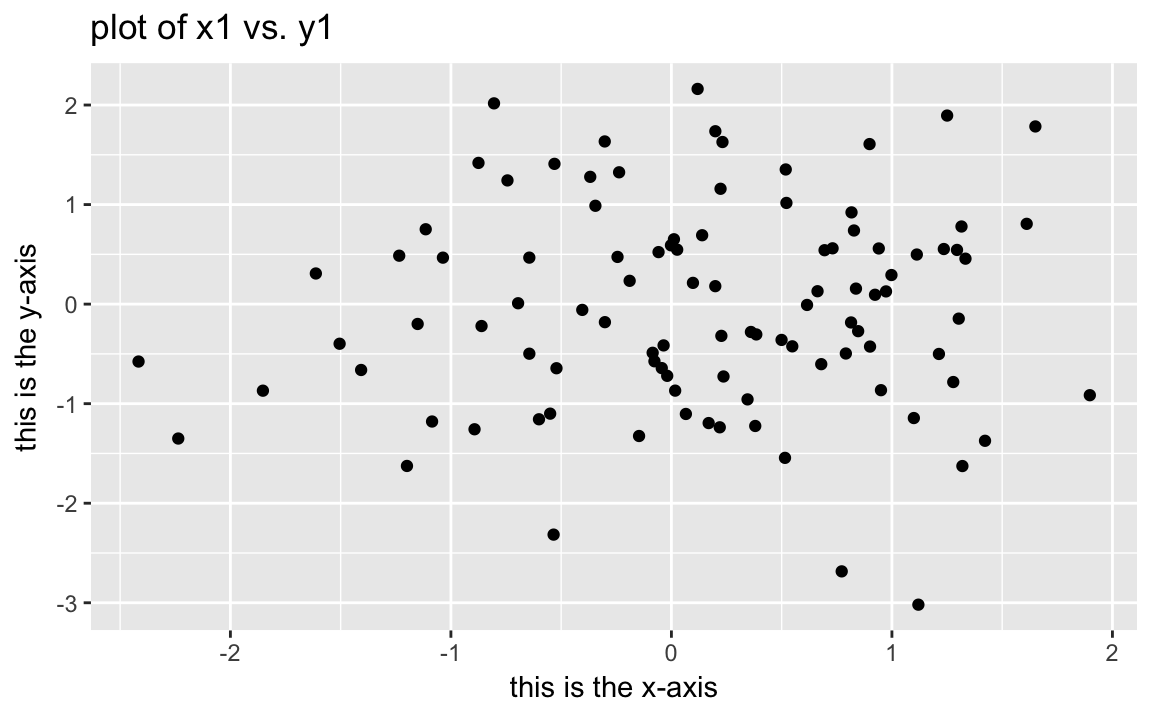
\includegraphics{tidy_islr_files/figure-latex/unnamed-chunk-1-1} \end{center}

\hypertarget{indexing-data}{%
\subsubsection{Indexing data}\label{indexing-data}}

We will skip this.

\hypertarget{loading-data}{%
\subsubsection{Loading data}\label{loading-data}}

\emph{ISLR} mentions insuring proper working directory before loading data. Dealing with working directories in R is a bad idea. Fortunately, it's easily avoidable through the use of RStudio \emph{projects}, which keep all files used in analysis together and make your work more robust and reproducible. See the \href{http://r4ds.had.co.nz/workflow-projects.html}{RStudio Projects} chapter in \emph{r4ds} for more information.

We will opt for the \texttt{readr} (part of the \texttt{tidyverse}) package instead of base R. Take a look at this subsection of \emph{r4ds} for reasons why:
\href{http://r4ds.had.co.nz/data-import.html}{\emph{11.2.1 Compared to base R}}

Below is a reproducible example in which we create a tibble, save it as a .txt file, and then read it in with \texttt{write\_tsv()}. The set of \texttt{read\_*} functions in \texttt{readr} will be the standrad way to read local files into R. If you are using RStudio projects, there is no need to worry about working directories.

\begin{Shaded}
\begin{Highlighting}[]
\CommentTok{# generate dummy data to read in}
\NormalTok{generic_company_tibble <-}\StringTok{ }\KeywordTok{tibble}\NormalTok{(}
  \DataTypeTok{x =} \KeywordTok{rnorm}\NormalTok{(}\DecValTok{100}\NormalTok{, }\DataTypeTok{mean =} \DecValTok{25}\NormalTok{),}
  \DataTypeTok{y =} \KeywordTok{rnorm}\NormalTok{(}\DecValTok{100}\NormalTok{, }\DataTypeTok{mean =} \DecValTok{50}\NormalTok{),}
  \DataTypeTok{z =} \KeywordTok{sample}\NormalTok{(}\KeywordTok{c}\NormalTok{(}\StringTok{"apple"}\NormalTok{, }\StringTok{"uber"}\NormalTok{, }\StringTok{"facebook"}\NormalTok{, }\StringTok{"twitter"}\NormalTok{, }\StringTok{"tesla"}\NormalTok{, }\StringTok{"google"}\NormalTok{, }\StringTok{"microsoft"}\NormalTok{), }\DecValTok{1}\NormalTok{)}
\NormalTok{)}

\NormalTok{tmp <-}\StringTok{ }\KeywordTok{tempfile}\NormalTok{()}
\KeywordTok{write_tsv}\NormalTok{(generic_company_tibble, tmp)}
\NormalTok{company_data <-}\StringTok{ }\KeywordTok{read_tsv}\NormalTok{(tmp)}
\end{Highlighting}
\end{Shaded}

\texttt{readr} provides a nice summary of the imported tibble. Calling the tibble by name will also give a breakdown of column names, data types, and number of observations.

\begin{Shaded}
\begin{Highlighting}[]
\NormalTok{company_data}
\end{Highlighting}
\end{Shaded}

\begin{verbatim}
## # A tibble: 100 x 3
##       x     y z     
##   <dbl> <dbl> <chr> 
## 1  23.0  50.1 google
## 2  23.7  50.3 google
## 3  25.8  48.9 google
## 4  24.5  51.5 google
## 5  24.6  48.2 google
## 6  23.8  49.8 google
## # ... with 94 more rows
\end{verbatim}

\hypertarget{additional-graphical-and-numerical-summaries}{%
\subsubsection{Additional Graphical and Numerical Summaries}\label{additional-graphical-and-numerical-summaries}}

ISLR mentions the \texttt{attach()} function, which allows R to reference column names of dataframes without specifying the dataframe. \texttt{attach} can lead to confusion and errors when working on a project with multiple sources of data. This is a bad practice, and should always be avoided.

The book then goes into some explanation of \texttt{plot()}, which we will not be using.

\begin{center}\rule{0.5\linewidth}{\linethickness}\end{center}

\hypertarget{exercises}{%
\section{Exercises}\label{exercises}}

\begin{enumerate}
\def\labelenumi{\arabic{enumi}.}
\tightlist
\item
  For each of parts (a) through (d), indicate whether we would generally expect the performance of a flexible statistical learning method to be better or worse than an inflexible method.

  \begin{enumerate}
  \def\labelenumii{(\alph{enumii})}
  \tightlist
  \item
    The sample size n is extremely large, and the number of predictors p is small

    \begin{itemize}
    \tightlist
    \item
      \textbf{(better)} given large sample size, a flexible model would be able to capture a trend without being influenced too heavily by a small number of observations.
    \end{itemize}
  \item
    The number of predictors p is extremely large, and the number of observations n is small.

    \begin{itemize}
    \tightlist
    \item
      \textbf{(worse)} given the small sample size, an inflexible model would do better at not overfitting to a small number of observations (capturing patterns in the training data that dont really exist)
    \end{itemize}
  \item
    The relationship between the predictors and response is highly non-linear.

    \begin{itemize}
    \tightlist
    \item
      \textbf{(better)} highly flexible methods are highly non-linear and can produce better fits on non-linear data compared to inflexible methods such as linear regression
    \end{itemize}
  \item
    The variance of the error terms, i.e.~σ2 = Var(ε), is extremely high.

    \begin{itemize}
    \tightlist
    \item
      \textbf{(worse)} given the high variance in the data, an inflexible method would overfit to the noise
    \end{itemize}
  \end{enumerate}
\item
  Explain whether each scenario is a classification or regression problem, and indicate whether we are most interested in inference or prediction. Finally, provide n and p.
\end{enumerate}

\begin{enumerate}
\def\labelenumi{(\alph{enumi})}
\tightlist
\item
  We collect a set of data on the top 500 firms in the US. For each firm we record profit, number of employees, industry and the CEO salary. We are interested in understanding which factors affect CEO salary.

  \begin{itemize}
  \tightlist
  \item
    \textbf{(regression; inference)} This is a regression problem with both qualitative and quantitative predictors. Inference is the main goal, as the company probably wants a model that is human-readable in order to understand what determines a CEO's salary.

    \begin{itemize}
    \tightlist
    \item
      \texttt{n\ =\ 500,\ p\ =\ 3}
    \end{itemize}
  \end{itemize}
\item
  We are considering launching a new product and wish to know whether it will be a success or a failure. We collect data on 20 similar products that were previously launched. For each product we have recorded whether it was a success or failure, price charged for the product, marketing budget, competition price, and ten other variables.

  \begin{itemize}
  \tightlist
  \item
    \textbf{(classification; prediction)} The goal is to classify whether a product will be a success or failure. Prediction is the goal, as they want to accurately determine if their product will succeed or fail.

    \begin{itemize}
    \tightlist
    \item
      \texttt{n\ =\ 20,\ p\ =\ 4}
    \end{itemize}
  \end{itemize}
\item
  We are interested in predicting the \% change in the USD/Euro exchange rate in relation to the weekly changes in the world stock markets. Hence we collect weekly data for all of 2012. For each week we record the \% change in the USD/Euro, the \% change in the US market, the \% change in the British market, and the \% change in the German market.

  \begin{itemize}
  \tightlist
  \item
    \textbf{(regression; prediction)} The goal is to predict the \% change of the exchange rate.
  \end{itemize}
\end{enumerate}

\begin{enumerate}
\def\labelenumi{\arabic{enumi}.}
\setcounter{enumi}{2}
\tightlist
\item
  We now revisit the bias-variance decomposition
\end{enumerate}

\begin{enumerate}
\def\labelenumi{(\alph{enumi})}
\tightlist
\item
  Provide a sketch of typical (squared) bias, variance, training error, test error, and Bayes (or irreducible) error curves, on a single plot, as we go from less flexible statistical learning methods towards more flexible approaches. The x-axis should represent the amount of flexibility in the method, and the y-axis should represent the values for each curve. There should be five curves. Make sure to label each one.
\end{enumerate}

\begin{Shaded}
\begin{Highlighting}[]
\NormalTok{bias_variance <-}\StringTok{ }\KeywordTok{tibble}\NormalTok{(}
  \DataTypeTok{flexibility =} \KeywordTok{c}\NormalTok{(}\DecValTok{1}\OperatorTok{:}\DecValTok{5}\NormalTok{),}
  \DataTypeTok{bias =} \KeywordTok{c}\NormalTok{(}\DecValTok{300}\NormalTok{,}\DecValTok{200}\NormalTok{,}\DecValTok{150}\NormalTok{,}\DecValTok{100}\NormalTok{,}\DecValTok{50}\NormalTok{),}
  \DataTypeTok{variance =} \KeywordTok{c}\NormalTok{(}\DecValTok{0}\NormalTok{,}\DecValTok{25}\NormalTok{,}\DecValTok{125}\NormalTok{,}\DecValTok{250}\NormalTok{,}\DecValTok{500}\NormalTok{),}
  \DataTypeTok{train_error =} \KeywordTok{c}\NormalTok{(}\DecValTok{350}\NormalTok{,}\DecValTok{250}\NormalTok{,}\DecValTok{200}\NormalTok{, }\DecValTok{125}\NormalTok{, }\DecValTok{50}\NormalTok{),}
  \DataTypeTok{irreducible_error =} \DecValTok{100}\NormalTok{,}
  \DataTypeTok{test_error =}\NormalTok{ variance }\OperatorTok{+}\StringTok{ }\NormalTok{bias }\OperatorTok{+}\StringTok{ }\NormalTok{irreducible_error) }\OperatorTok
\StringTok{  }\KeywordTok{gather}\NormalTok{(}\StringTok{`}\DataTypeTok{bias}\StringTok{`}\NormalTok{, }\StringTok{`}\DataTypeTok{variance}\StringTok{`}\NormalTok{, }\StringTok{`}\DataTypeTok{train_error}\StringTok{`}\NormalTok{, }\StringTok{`}\DataTypeTok{irreducible_error}\StringTok{`}\NormalTok{, }\StringTok{`}\DataTypeTok{test_error}\StringTok{`}\NormalTok{,}
         \DataTypeTok{key =} \StringTok{"measurement"}\NormalTok{, }\DataTypeTok{value =} \StringTok{"value"}\NormalTok{)}

\KeywordTok{ggplot}\NormalTok{(bias_variance, }\KeywordTok{aes}\NormalTok{(}\DataTypeTok{x =}\NormalTok{ flexibility, }\DataTypeTok{y =}\NormalTok{ value, }\DataTypeTok{colour =}\NormalTok{ measurement)) }\OperatorTok{+}
\StringTok{  }\KeywordTok{geom_smooth}\NormalTok{(}\DataTypeTok{se =} \OtherTok{FALSE}\NormalTok{, }\DataTypeTok{method =} \StringTok{"lm"}\NormalTok{, }\DataTypeTok{formula =}\NormalTok{ y }\OperatorTok{~}\StringTok{ }\KeywordTok{poly}\NormalTok{(x,}\DecValTok{3}\NormalTok{)) }\OperatorTok{+}
\StringTok{  }\KeywordTok{theme_minimal}\NormalTok{()}
\end{Highlighting}
\end{Shaded}

\begin{center}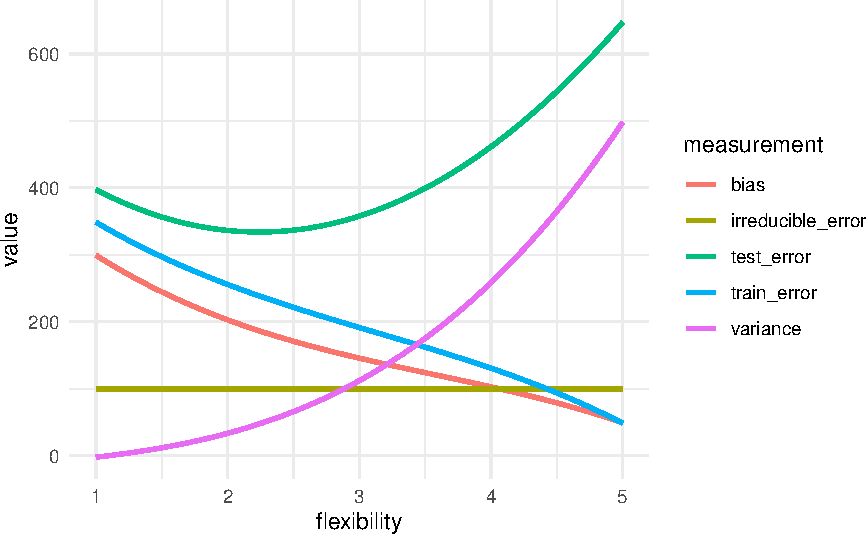
\includegraphics{tidy_islr_files/figure-latex/unnamed-chunk-4-1} \end{center}

\begin{enumerate}
\def\labelenumi{\arabic{enumi}.}
\setcounter{enumi}{3}
\tightlist
\item
  You will now think of some real-life applications for statistical learning.

  \begin{enumerate}
  \def\labelenumii{(\alph{enumii})}
  \tightlist
  \item
    Describe three real-life applications in which classification might be useful. Describe the response, as well as the predictors. Is the goal of each application inference or prediction? Explain your answer.

    \begin{enumerate}
    \def\labelenumiii{\arabic{enumiii}.}
    \tightlist
    \item
      predicting diabetes.

      \begin{itemize}
      \tightlist
      \item
        response: future diabetes
      \item
        predictors: health and body measurements of patient
      \item
        goal: prediction, model complexity and human understanding is not important
      \end{itemize}
    \item
      demographics that determine future education level

      \begin{itemize}
      \tightlist
      \item
        response: education level
      \item
        predictors: demographic data
      \item
        goal: inference, prediction is important here too but researchers would probably want to understand and share which factors determine the response in order to raise awareness
      \end{itemize}
    \item
      faulty parts in manufacturing

      \begin{itemize}
      \tightlist
      \item
        response: whether or not part is faulty
      \item
        predictors: various tests on part
      \item
        goal: prediction, it is most important to have an accurate model, especially if faulty parts can lead to deaths
      \end{itemize}
    \end{enumerate}
  \item
    Describe three real-life applications in which regression might be useful. Describe the response, as well as the predictors. Is the goal of each application inference or prediction? Explain your answer.

    \begin{enumerate}
    \def\labelenumiii{\arabic{enumiii}.}
    \tightlist
    \item
      number of riders on public transit over time

      \begin{itemize}
      \tightlist
      \item
        response: how many riders are expected to use public transit
      \item
        predictors: current transit usage data, local population data, etc.
      \item
        goal: prediction, it is important to prepare for growth in transit usage so governments have enough time to make necessary changes
      \end{itemize}
    \item
      demand for product

      \begin{itemize}
      \tightlist
      \item
        response: how many units to expect to be sold
      \item
        predictors: current demand data, revenue growth, business expansion, changing in market trends, economy health
      \item
        goal: prediction, figure out in X amount of time demand for product in order to upsize/downsize to appropriate level
      \end{itemize}
    \item
      determine future salary

      \begin{itemize}
      \tightlist
      \item
        response: future expeceted salary
      \item
        predictors: employment history, education, geolocation, etc.
      \item
        goal: inference, researchers might want to know the most important factors that lead to higher salaries rather than a model that is too complex to understand
      \end{itemize}
    \end{enumerate}
  \end{enumerate}
\item
  What are the advantages and disadvantages of a very flexible (versus a less flexible) approach for regression or classification? Under what circumstances might a more flexible approach be preferred to a less flexible approach? When might a less flexible approach be preferred?
\end{enumerate}

\begin{itemize}
\tightlist
\item
  Very flexible approach allows you to fit a more flexible function to the data. The advantage is that you have the potential to accurately predict data even as it moves away from linearity. The disadvantage are potential overfitting to the training data, increasing variance (individual observations affect the model to higher degree than non-flexible counterpart), and higher computational costs (as well as less human-readable explanations)
\item
  When a more flexible approach is preferred: data that is non-linear, large sample size, prediction more important than inference
\item
  When a less flexible approach is preferred: data that is more linear, smaller sample size, inference more important than prediction
\end{itemize}

\begin{enumerate}
\def\labelenumi{\arabic{enumi}.}
\setcounter{enumi}{5}
\tightlist
\item
  Describe the differences between a parametric and a non-parametric statistical learning approach. What are the advantages of a parametric approach to regression or classification (as opposed to a nonparametric approach)? What are its disadvantages?
\end{enumerate}

\begin{itemize}
\tightlist
\item
  A parametric approach assumes a form of \(f\) and has to estimate an often known number of parameters (for example, linear regression simply requires estimating \(p+1\) coefficients)
\item
  A non-parametric approach makes no assumptions about the true form of \(f\). They simply want to get as close as possible to \(f\). This allows them to take on a larger variety of shapes, and accomodate a larger variety of patterns.
\item
  Advantages of a parametric approach are that they take less observations to generate (the problem is reduced to applying a known form to \(f\), such as linear regression), are less inclined to overfit, and generally less computationally intensive.
\item
  Disadvantages of a parametric approach making assumptions about the form of \(f\), which may not match the real form and could lead to a model that doesn't fit the data well
\end{itemize}

\begin{enumerate}
\def\labelenumi{\arabic{enumi}.}
\setcounter{enumi}{6}
\tightlist
\item
  The table below provides a training data set containing six observa- tions, three predictors, and one qualitative response variable.
\end{enumerate}

\begin{Shaded}
\begin{Highlighting}[]
\NormalTok{training_set <-}\StringTok{ }\KeywordTok{tibble}\NormalTok{(}
  \DataTypeTok{x1 =} \KeywordTok{c}\NormalTok{(}\DecValTok{0}\NormalTok{,}\DecValTok{2}\NormalTok{,}\DecValTok{0}\NormalTok{,}\DecValTok{0}\NormalTok{,}\OperatorTok{-}\DecValTok{1}\NormalTok{,}\DecValTok{1}\NormalTok{),}
  \DataTypeTok{x2 =} \KeywordTok{c}\NormalTok{(}\DecValTok{3}\NormalTok{,}\DecValTok{0}\NormalTok{,}\DecValTok{1}\NormalTok{,}\DecValTok{1}\NormalTok{,}\DecValTok{0}\NormalTok{,}\DecValTok{1}\NormalTok{),}
  \DataTypeTok{x3 =} \KeywordTok{c}\NormalTok{(}\DecValTok{0}\NormalTok{,}\DecValTok{0}\NormalTok{,}\DecValTok{3}\NormalTok{,}\DecValTok{2}\NormalTok{,}\DecValTok{1}\NormalTok{,}\DecValTok{1}\NormalTok{),}
  \DataTypeTok{y =} \KeywordTok{c}\NormalTok{(}\StringTok{"red"}\NormalTok{,}\StringTok{"red"}\NormalTok{,}\StringTok{"red"}\NormalTok{,}\StringTok{"green"}\NormalTok{,}\StringTok{"green"}\NormalTok{,}\StringTok{"red"}\NormalTok{))}

\KeywordTok{kable}\NormalTok{(training_set)}
\end{Highlighting}
\end{Shaded}

x1

x2

x3

y

0

3

0

red

2

0

0

red

0

1

3

red

0

1

2

green

-1

0

1

green

1

1

1

red

Suppose we wish to use this data set to make a prediction for \(Y\) when \(X1 = X2 = X3 = 0\) using K-nearest neighbors.

\begin{enumerate}
\def\labelenumi{(\alph{enumi})}
\tightlist
\item
  Compute the Euclidean distance between each observation and the test point, \(X1 = X2 = X3 = 0\).
\end{enumerate}

The Euclidean Distance for three dimensions can be written as:

\(d = \sqrt {\left( {x_1 - x_2 } \right)^2 + \left( {y_1 - y_2 } \right)^2 + \left( {z_1 - z_2 } \right)^2 }\)

Let's write a function that can handle this in R, then use the \texttt{rowwise()} feature of dplyr to apply it across the rows of our tibble.

\begin{Shaded}
\begin{Highlighting}[]
\NormalTok{euc_dist <-}\StringTok{ }\ControlFlowTok{function}\NormalTok{(x1, x2) }\KeywordTok{sqrt}\NormalTok{(}\KeywordTok{sum}\NormalTok{((x1 }\OperatorTok{-}\StringTok{ }\NormalTok{x2) }\OperatorTok{^}\StringTok{ }\DecValTok{2}\NormalTok{))}
\NormalTok{training_set <-}\StringTok{ }\NormalTok{training_set }\OperatorTok
\StringTok{  }\KeywordTok{rowwise}\NormalTok{() }\OperatorTok
\StringTok{  }\KeywordTok{mutate}\NormalTok{(}\DataTypeTok{distance =} \KeywordTok{euc_dist}\NormalTok{(}\KeywordTok{c}\NormalTok{(x1,x2,x3), }\KeywordTok{c}\NormalTok{(}\DecValTok{0}\NormalTok{,}\DecValTok{0}\NormalTok{,}\DecValTok{0}\NormalTok{))) }\OperatorTok
\StringTok{  }\KeywordTok{ungroup}\NormalTok{()}

\KeywordTok{kable}\NormalTok{(training_set)}
\end{Highlighting}
\end{Shaded}

x1

x2

x3

y

distance

0

3

0

red

3.000000

2

0

0

red

2.000000

0

1

3

red

3.162278

0

1

2

green

2.236068

-1

0

1

green

1.414214

1

1

1

red

1.732051

\begin{enumerate}
\def\labelenumi{(\alph{enumi})}
\setcounter{enumi}{1}
\tightlist
\item
  What is our prediction with K = 1? Why?
\end{enumerate}

Let's find the \texttt{y} value of the single closest (\texttt{k\ =\ 1}) training observation.

\begin{Shaded}
\begin{Highlighting}[]
\NormalTok{training_set }\OperatorTok\StringTok{ }
\StringTok{  }\KeywordTok{filter}\NormalTok{(distance }\OperatorTok{==}\StringTok{ }\KeywordTok{min}\NormalTok{(distance)) }\OperatorTok
\StringTok{  }\KeywordTok{select}\NormalTok{(y) }\OperatorTok
\StringTok{  }\KeywordTok{pull}\NormalTok{()}
\end{Highlighting}
\end{Shaded}

\begin{verbatim}
## [1] "green"
\end{verbatim}

Since the closest observation in the training data is \texttt{green}, \texttt{K\ =\ 1} classifies our test observation as \texttt{green}.

\begin{enumerate}
\def\labelenumi{(\alph{enumi})}
\setcounter{enumi}{2}
\tightlist
\item
  What is our prediction with K = 3? Why?
\end{enumerate}

First we find the three closest values. Then we measure the breakdown of \texttt{y} responses in this group of three observations. We find that two observations have value of \texttt{red}, and one has \texttt{green}. Given \texttt{red} has the highest probability of the two \texttt{y} values, we assign the training observation as \texttt{red}.

\begin{Shaded}
\begin{Highlighting}[]
\NormalTok{training_set }\OperatorTok
\StringTok{  }\KeywordTok{top_n}\NormalTok{(}\DecValTok{3}\NormalTok{, }\OperatorTok{-}\NormalTok{distance) }\OperatorTok
\StringTok{  }\KeywordTok{mutate}\NormalTok{(}\DataTypeTok{n =} \KeywordTok{n}\NormalTok{()) }\OperatorTok
\StringTok{  }\KeywordTok{group_by}\NormalTok{(y) }\OperatorTok
\StringTok{  }\KeywordTok{summarise}\NormalTok{(}\DataTypeTok{prop =} \KeywordTok{n}\NormalTok{()}\OperatorTok{/}\KeywordTok{max}\NormalTok{(n)) }\OperatorTok
\StringTok{  }\KeywordTok{filter}\NormalTok{(prop }\OperatorTok{==}\StringTok{ }\KeywordTok{max}\NormalTok{(prop)) }\OperatorTok
\StringTok{  }\KeywordTok{pull}\NormalTok{(y)}
\end{Highlighting}
\end{Shaded}

\begin{verbatim}
## [1] "red"
\end{verbatim}

\begin{enumerate}
\def\labelenumi{(\alph{enumi})}
\setcounter{enumi}{3}
\tightlist
\item
  If Bayes decision boundary is highly non-linear, then do we expect the best value of \(K\) to be large or small? Why?

  \begin{itemize}
  \tightlist
  \item
    We expect the value of \(K\) to decline as the decision boundary grows more non-linear. A smaller value of \(K\) is more suspectible to small changes between observations, which is the type of pattern highly non-linear decision boundary would depict.
  \end{itemize}
\end{enumerate}

The R exercises are pretty basic after this. I am going to skip them for now.

\hypertarget{linear-regression}{%
\chapter{Linear Regression}\label{linear-regression}}

\begin{center}\rule{0.5\linewidth}{\linethickness}\end{center}

Linear regression is a simple yet very powerful approach in statistical learning. It is important to have a strong understanding of it before moving on to more complex learning methods.

\hypertarget{simple-linear-regression}{%
\section{Simple Linear Regression}\label{simple-linear-regression}}

Simple linear regression is predicting a quantitative response \(Y\) based off a single predcitor \(X\).

It can be written as below:

\(Y \approx \beta_0 + \beta_1X\)

\emph{simple linear regression}

\(\beta_0\) and \(\beta_1\) represent the \emph{intercept} and \emph{slope} terms and are together known as the \emph{coefficients}.
\(\beta_0\) and \(\beta_1\) represent the unknown \emph{intercept} and \emph{slope} terms and are together known as the \emph{coefficients}. We will use our training data to estimate these parameters and thus estimate the response \(Y\) based on the value of \(X = x\):

\(\hat y = \hat\beta_0 + \hat\beta_1x\)

\hypertarget{estimating-the-coefficients}{%
\subsection{Estimating the Coefficients}\label{estimating-the-coefficients}}

We need to use data to estimate these coefficients.

\((x_1,y_1), (x_2,y_2),..., (x_n,y_n)\)

These represent the training observations, in this case pairs of \(X\) and \(Y\) measurements. The goal is to use these measurements to estimate \(\beta_0\) and \(\beta_1\) such that the linear model fits our data as close as possible. Measuring \emph{closeness} can be tackled a number of ways, but \href{https://en.wikipedia.org/wiki/Least_squares}{least squares} is the most popular.

If we let \(\hat y_i = \hat\beta_0 + \hat\beta_1x_i\) be the prediction of \(Y\) at observation \(X_i\), then \(e_i = y_i - \hat y_i\) represents the \(i\)th \emph{residual}, the difference between the observed value \(y_i\) and the predicted value \(\hat y_i\). Now we can define the \emph{residual sum of squares (RSS)} as

\(RSS = e_1^2 + e_2^2 + ... + e_n^2\)

\emph{residual sum of squares}

or more explicitly as

\(RSS = (y_1 - \hat\beta_0 - \hat\beta_1x_2)^2 + (y_2 - \hat\beta_0 - \hat\beta_1x_2)^2 + ... + (y_n - \hat\beta_0 - \hat\beta_1x_n)^2\)

Minimizing the RSS (proof can be found \href{https://en.m.wikipedia.org/wiki/Simple_linear_regression\#Derivation_of_simple_regression_estimators}{here}) using \(\beta_0\) and \(\beta_1\) produces:

\(\frac{\displaystyle \sum_{i=1}^{n}(x_i-\bar x)(y_i - \bar x)}{\displaystyle\sum_{i=1}^{n}(x_i - \bar x)^2}\)

\emph{least squares coefficient estimates (simple linear regression)}

\hypertarget{assessing-the-accuracy-of-the-coefficient-estimate}{%
\subsection{Assessing the Accuracy of the Coefficient Estimate}\label{assessing-the-accuracy-of-the-coefficient-estimate}}

Remember that the true function for \(f\) contains a random error term \(\epsilon\). This means the linear relationship can be written as

\(Y = \beta_0 + \beta_1X + \epsilon\)

\emph{population regression line}

\(\beta_0\) is the intercept term (value of \(Y\) when \(X = 0\)). \(\beta_1\) is the slope (how much does \(Y\) change with one-unit change of \(X\)). \(\epsilon\) is the error term that captures everything our model doesn't (unknown variables, measurement error, unknown true relationship).

The population regression line captures the best linear approximation to the true relationship between \(X\) and \(Y\). In real data, we often don't know the true relationship and have to rely on a set of observations. Using the observations to estimate the coefficients via least squares produces the \emph{least squares line}. Let's simulate and visualize this relationship:

\begin{itemize}
\tightlist
\item
  simulate \texttt{n\ =\ 200} observations

  \begin{itemize}
  \tightlist
  \item
    compare the population regression line (\texttt{sim\_y}) to a number of possible least squares lines (generated from 10 different training sets of the data)
  \end{itemize}
\end{itemize}

\begin{Shaded}
\begin{Highlighting}[]
\CommentTok{# f(x), or Y = 2 + 2x + error}

\NormalTok{sim_linear <-}\StringTok{ }\KeywordTok{tibble}\NormalTok{(}
  \DataTypeTok{b0 =} \DecValTok{2}\NormalTok{,}
  \DataTypeTok{b1 =} \DecValTok{2}\NormalTok{,}
  \DataTypeTok{x =} \DecValTok{1}\OperatorTok{:}\DecValTok{100} \OperatorTok{+}\StringTok{ }\KeywordTok{rnorm}\NormalTok{(}\DataTypeTok{n =} \DecValTok{200}\NormalTok{, }\DataTypeTok{mean =} \DecValTok{100}\NormalTok{, }\DataTypeTok{sd =} \DecValTok{15}\NormalTok{),}
  \DataTypeTok{err =} \KeywordTok{rnorm}\NormalTok{(}\DecValTok{200}\NormalTok{, }\DataTypeTok{sd =} \DecValTok{50}\NormalTok{),}
  \DataTypeTok{sim_y =}\NormalTok{ b0 }\OperatorTok{+}\StringTok{ }\NormalTok{b1 }\OperatorTok{*}\StringTok{ }\NormalTok{x,}
  \DataTypeTok{true_y =}\NormalTok{ b0 }\OperatorTok{+}\StringTok{ }\NormalTok{b1}\OperatorTok{*}\NormalTok{x }\OperatorTok{+}\StringTok{ }\NormalTok{err}
\NormalTok{)}

\CommentTok{# generate 10 training sets}
\NormalTok{y <-}\StringTok{ }\KeywordTok{tibble}\NormalTok{()}
\ControlFlowTok{for}\NormalTok{ (i }\ControlFlowTok{in} \DecValTok{1}\OperatorTok{:}\DecValTok{10}\NormalTok{) \{}
\NormalTok{x <-}\StringTok{ }\KeywordTok{sample_frac}\NormalTok{(sim_linear, }\FloatTok{0.1}\NormalTok{) }\OperatorTok\StringTok{ }\KeywordTok{mutate}\NormalTok{(}\DataTypeTok{iter_set =}\NormalTok{ i)}
\NormalTok{y <-}\StringTok{ }\NormalTok{y }\OperatorTok\StringTok{ }\KeywordTok{bind_rows}\NormalTok{(x)}
\NormalTok{\}}

\CommentTok{# apply linear model to each sample}
\NormalTok{by_iter <-}\StringTok{ }\NormalTok{y }\OperatorTok
\StringTok{  }\KeywordTok{group_by}\NormalTok{(iter_set) }\OperatorTok
\StringTok{  }\KeywordTok{nest}\NormalTok{()}
\NormalTok{lm_model <-}\StringTok{ }\ControlFlowTok{function}\NormalTok{(df) \{}
  \KeywordTok{lm}\NormalTok{(true_y }\OperatorTok{~}\StringTok{ }\NormalTok{x, }\DataTypeTok{data =}\NormalTok{ df)}
\NormalTok{\}}
\NormalTok{by_iter <-}\StringTok{ }\NormalTok{by_iter }\OperatorTok
\StringTok{  }\KeywordTok{mutate}\NormalTok{(}\DataTypeTok{model =} \KeywordTok{map}\NormalTok{(data, lm_model),}
         \DataTypeTok{preds =} \KeywordTok{map2}\NormalTok{(data, model, add_predictions))}

\CommentTok{# extract predictions}
\NormalTok{preds <-}\StringTok{ }\KeywordTok{unnest}\NormalTok{(by_iter, preds)}

\KeywordTok{ggplot}\NormalTok{(}\DataTypeTok{data =}\NormalTok{ sim_linear, }\KeywordTok{aes}\NormalTok{(}\DataTypeTok{x =}\NormalTok{ x, }\DataTypeTok{y =}\NormalTok{ true_y)) }\OperatorTok{+}
\StringTok{  }\KeywordTok{geom_point}\NormalTok{(}\DataTypeTok{alpha =} \DecValTok{1}\OperatorTok{/}\DecValTok{3}\NormalTok{) }\OperatorTok{+}
\StringTok{  }\KeywordTok{geom_line}\NormalTok{(}\DataTypeTok{data =}\NormalTok{ preds, }\KeywordTok{aes}\NormalTok{(}\DataTypeTok{x =}\NormalTok{ x, }\DataTypeTok{y =}\NormalTok{ pred, }\DataTypeTok{colour =}\NormalTok{ iter_set, }\DataTypeTok{group =}\NormalTok{ iter_set), }\DataTypeTok{linetype =} \StringTok{"F1"}\NormalTok{, }\DataTypeTok{size =} \FloatTok{.75}\NormalTok{) }\OperatorTok{+}
\StringTok{  }\KeywordTok{geom_line}\NormalTok{(}\KeywordTok{aes}\NormalTok{(}\DataTypeTok{y =}\NormalTok{ sim_y), }\DataTypeTok{colour =} \StringTok{"red"}\NormalTok{, }\DataTypeTok{size =} \FloatTok{1.5}\NormalTok{) }\OperatorTok{+}
\StringTok{  }\KeywordTok{theme_minimal}\NormalTok{() }\OperatorTok{+}
\StringTok{  }\KeywordTok{theme}\NormalTok{(}\DataTypeTok{legend.position =} \StringTok{"none"}\NormalTok{, }\DataTypeTok{panel.grid.minor =} \KeywordTok{element_blank}\NormalTok{(),}
        \DataTypeTok{panel.grid.major =} \KeywordTok{element_blank}\NormalTok{(), }\DataTypeTok{axis.line =} \KeywordTok{element_line}\NormalTok{(}\DataTypeTok{colour =} \StringTok{"grey92"}\NormalTok{)) }\OperatorTok{+}
\StringTok{  }\KeywordTok{labs}\NormalTok{(}\DataTypeTok{title =} \StringTok{"Each least squares line provides a reasonable estimate"}\NormalTok{,}
       \DataTypeTok{y =} \StringTok{"y"}\NormalTok{)}
\end{Highlighting}
\end{Shaded}

\begin{center}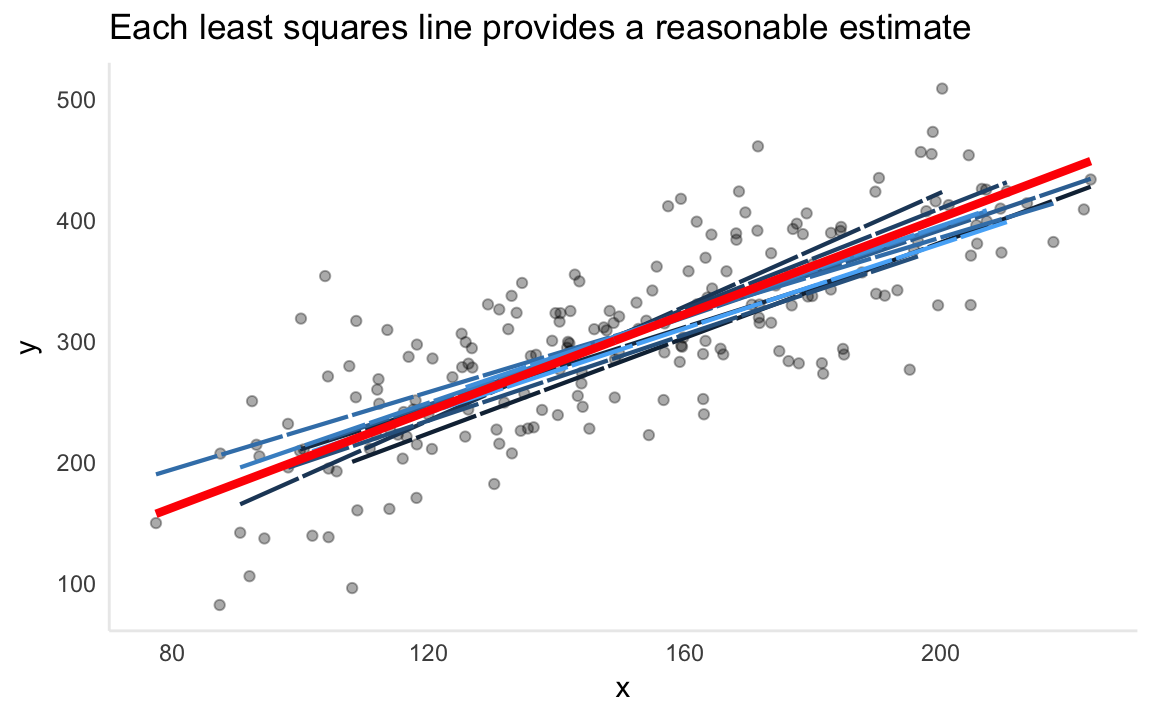
\includegraphics{tidy_islr_files/figure-latex/unnamed-chunk-9-1} \end{center}

The chart above demonstrates the population regression line (red) surrounded by ten different estimates of the least squares line. Notice how every least squares line (shades of blue) is different. This is because each one is generated from a random sample pulled from the simulated data. For a real-world comparison, the simulated data would be the entire population data which is often impossible to obtain. The observations used to generate the least squares line would be the sample data we have access to. In the same way a sample mean can provide a reasonable estimate of the population mean, fitting a least squares line can provide a reasonable estimate of the population regression line.

This comparison of linear regression to estimating population means touches on the topic of bias. An estimate of \(\mu\) using the the sample mean \(\hat\mu\) is unbiased. On average, the sample mean will not systemically over or underestimate \(\mu\). If we were to take a large enough estimates of \(\mu\), each produced by a particular set of observations, then this average would exactly equal \(\mu\). This concept applies to our estimates of \(\beta_0, \beta_1\) as well.

A question that can be asked is how close on average the sample mean \(\hat\mu\) is to \(\mu\). We can compute the \emph{standard error} of \(\hat\mu\) to answer this.

\(Var(\hat\mu) = SE(\hat\mu)^2 = \sigma^2/n\)

\emph{standard error}

This formula measures the average amount that \(\hat\mu\) differs from \(\mu\). As the number of observations \(n\) increases, the standard error decreases.

We can also use this to calculate how close \(\hat\beta_0, \hat\beta_1\) are to \(\beta_0, \beta_1\).

\(SE(\hat\beta_0)^2= \sigma^2 \left[1/n + \frac{\displaystyle \bar x^2}{\displaystyle\sum_{i=1}^{n}(x_i - \bar x)^2} \right]\)

\(SE(\hat\beta_1)^2=\frac{\displaystyle \sigma^2}{\displaystyle\sum_{i=1}^{n}(x_i - \bar x)^2}\)

where \(\sigma^2 = Var(\epsilon)\). For this to work, the assumption has to be made that the error terms \(\epsilon_i\) are uncorrelated and all share a common variance. This is often not the case, but it doesn't mean the formula can't be used for a decent approximation. \(\sigma^2\) is not known, but can be estimated from training observations. This estimate is the \emph{residual standard error} and is given by formula \(RSE = \sqrt{RSS/(n-2}\).

What can we use these standard error formulas for? A useful technique is to calculate \emph{confidence intervals} from the standard error. If we wanted to compute a 95\% confidence interval for \(\beta_0,\beta_1\), it would take the form below.

\(\hat\beta_1 \pm 2 * SE(\hat\beta_1)\)

\(\hat\beta_0 \pm 2 * SE(\hat\beta_0)\)

Standard errors can also be used to perform hypotheses tests.

\(H_0\): There is no relationship between \(X\) and \(Y\), or \(\beta_1 = 0\)

\emph{null hypothesis}

\(H_0\): There exists a relationship between \(X\) and \(Y\), or \(\beta_1 \neq 0\)

\emph{alternative hypothesis}

To test the null hypothesis, we need to test whether \(\hat\beta_1\) is far enough away from zero to conclude that is it non-zero. How far enough from zero is determined by the value of \(\hat\beta_1\) as well as \(SE(\hat\beta_1)\). We compute a \emph{t-statistic}

\(t = (\beta_1 - 0)/SE(\hat\beta_1)\)

\emph{t-statistic}

This measures how many standard deviations \(\hat\beta_1\) is from 0. If there is no relationship between \(X\) and \(Y\), then \(t\) will follow a t-distribution. The t-distribution is similar to the normal distribution, but has slightly heavier tails. Like the normal distribution, we can use this to compute the probability of observing any number equal to or larger than \(|t|\). This probability is the \emph{p-value}. We can interpret a p-value as the probability we would observe the sample data that produced the \(t\)-statistic, given that there is no actual relationship between the predictor \(X\) and the response \(Y\). This means that a small p-value supports the inference that there exists a relationship between the predictor and the response. In this case, based on whichever threshold \(\alpha\) (common value is 0.05) we set, a small enough p-value would lead us to reject the null hypothesis.

\hypertarget{assessing-the-accuracy-of-the-model}{%
\subsection{Assessing the Accuracy of the Model}\label{assessing-the-accuracy-of-the-model}}

Now that we determined the existence of a relationship, how can we measure how well the model fits the data?

Measuring the quality of a linear regression fit is often handled by two quantities: the \emph{residual standard error} and the \emph{R\^{}2} statistic.

\hypertarget{residual-standard-error}{%
\subsubsection{Residual Standard Error}\label{residual-standard-error}}

Since every observation has an associated error term \(\epsilon\), having the knowledge of true \(\beta_0\) and \(\beta_1\) will still not allow one to perfectly predict \(Y\). The residual standard error estimates the standard deviation of the error term.

\(RSE = \sqrt{1/(n-2)*RSS} = \sqrt{1/(n-2)\sum_{i=1}^{n}(y_i - \hat y)^2}\)

\emph{residual standard error}

We can interpret the residual standard error as how much, on average, our predictions deviate from the true value. Whether the value is acceptable in terms of being a successful model depends on the context of the problem. Predicting hardware failure on an airplane would obviously carry much more stringent requirements than predicting the added sales from a change in a company's advertising budget.

\hypertarget{r2-statistic}{%
\subsubsection{R\^{}2 statistic}\label{r2-statistic}}

The RSE provides an absolute number. Given that it depends on the scale of \(Y\), comparing RSE values across different domains and datasets isn't useful. The R\^{}2 statistic solves this problem by measuring in terms of proportion -- it measures the variance explained and so always takes a value between 0 and 1.

\(R^2 = (TSS - RSS)/TSS = 1 - RSS/TSS\)

\emph{R\^{}2 statistic}

where \(TSS = \sum_{i=1}^{n}(y_i-\bar y)^2\) is the \emph{total sum of squares}. TSS can be thought of the amount of total variability in the response variable before any model is fitted to it. RSS is measured after fitting a model, and measures the amount of unexplained variance remaining in the data. Therefore, R\^{}2 can be thought of as the proportion of variance in the data that is explained by fitting a model with \(X\). While R\^{}2 is more intrepetable, determing what constitutes a R\^{}2 is subjective to the problem. Relationships that are known to be linear with little variance would expect an R\^{}2 very close to 1. In reality, a lot of real-world data is not truly linear and could be heavily influenced by unknown, immeasurable predictors. In such cases a linear approximation would be a rough fit, and a smaller R\^{}2 would not be unordinary.

There is a relation between R\^{}2 and the correlation.

\(r = Cor(X,Y) = \sum_{i=1}^{n}((x_i-\bar x)(y_i - \bar y))/(\sqrt{\sum_{i=1}^{n}(x_i - \bar x)^2}\sqrt{\sum_{i=1}^{n}(y_i - \bar y)^2})\)

\emph{correlation}

Both measure the linear relationship between \(X\) and \(Y\), and within the simple linear regression domain, \(r^2 = R^2\). Once we move into multiple linear regression, in which we are using multiple predictors to predict a response, correlation loses effectiveness at measuring a model in whole as it can only measure the relationship between a single pair of variables.

\hypertarget{multiple-linear-regression}{%
\section{Multiple Linear Regression}\label{multiple-linear-regression}}

Simple linear regression works well when the data involves a single predictor variable. In reality, there are often multiple predictor variables. We will need to extend the simple linear regression model and provide each predictor variable \(p\) with a slope coefficient.

\(Y = \beta_0 + \beta_1X_1 + \beta_2X_2 + ... + \beta_pX_p + \epsilon\)

\emph{multiple linear regression}

\hypertarget{estimating-the-regression-coefficients}{%
\subsection{Estimating the Regression Coefficients}\label{estimating-the-regression-coefficients}}

Again, we need to estimate the regression coefficients.

\(\hat y = \hat\beta_0 + \hat\beta_1X_1 + \hat\beta_2X_2 + ... + \hat\beta_pX_p\)

We will utilize the same approach of minimizing the sum of squared residuals (RSS).

\(RSS = \sum_{i=1}^{n}(y_i - \hat y_i)^2 = \sum_{i=1}^{n}(y_i - \hat\beta_0 - \hat\beta_1x_{i1} - \hat\beta_2x_{i2} - ... - \hat\beta_px_{ip})^2\)

Minimizing these coefficients is more complicated than the simple linear regression setting, and is best represented using linear algebra. See \href{https://en.wikipedia.org/wiki/Residual_sum_of_squares\#Matrix_expression_for_the_OLS_residual_sum_of_squares}{this Wikipedia section} for more information on the formula.

Interpreting a particular coefficient, (say \(\beta_1\)) in a multiple regression model can be thought of as follows: if constant value for all other \(\beta_p\) are maintained, what effect would an increase in \(beta_1\) have on \(Y\)?

A side effect of this is that certain predictors which were deemed significant when contained in a simple linear regression can become insignificant when multiple predictors are involved. For an advertising example, \texttt{newspaper} could be a significant predictor of \texttt{revenue} in the simple linear regression context. However, when combined with \texttt{tv} and \texttt{radio} in a multiple linear regression setting, the effects of increasing \texttt{newspaper} spend while maintaining \texttt{tv} and \texttt{radio} becomes insignificant. This could be due to a correlation of \texttt{newspaper} spend in markets where \texttt{radio} spend is high. Multiple linear regression exposes predictors that act as ``surrogates'' for others due to correlation.

\hypertarget{some-important-questions}{%
\subsection{Some Important Questions}\label{some-important-questions}}

\hypertarget{is-there-a-relationship-between-the-response-and-predictors}{%
\subsubsection{Is There a Relationship Between the Response and Predictors?}\label{is-there-a-relationship-between-the-response-and-predictors}}

To check this, we need to check whethere all \(p\) coefficients are zero, i.e. \(\beta_1 = \beta_2 = ... = \beta_p = 0\). We test the null hypothesis,

\(H_o:\beta_1 = \beta_2 = ... = \beta_p = 0\)

against the alternative

\(H_a:\) at least one \(\beta_j\) is non-zero

The hypothesis test is performed by computing the \(F-statistic\),

\(F = \frac{(TSS-RSS)/p}{RSS/(n-p-1)}\)

\emph{correlation}

If linear model assumptions are correct, one can show that

\(E\{RSS/(n-p-1)\} = \sigma^2\)

and that, provided \(H_o\) is true,

\(E\{(TSS-RSS)/p\} = \sigma^2\)

In simple terms, if \(H_o\) were true and all of the predictors have regression coefficients of 0, we would expect the unexplained variance of the model to be approximately equal to that of the total variance, and both the numerator and the denominator of the F-statistic formula to be equal. When there is no relationship between the response and predictors, the F-statistic will take on a value close to 1. However, as RSS shrinks (the model begins to account for more of the variance), the numerator grows and the denominator shrinks, both causing the F-statistic to increase. We can think of the F-statistic as a ratio between the explained variance and unexplained variance. As the explained variance grows larger than the unexplained portion, the likelihood that we reject the null hypothesis grows.

How large does the F-statistic need to be to reject the null hypothesis? This depends on \(n\) and \(p\). As \(n\) grows, F-statistics closer to 1 may provide sufficient evidence to reject \(H_o\). If \(H_o\) is true and \(\epsilon_i\) have a normal distribution, the F-statistic follows an F-distribution. We can compute the p-value for any value of \(n\) and \(p\) associated with an F-statistic.

Sometimes we want to test whether a particular subset of \(q\) of the coefficients are zero.

The null hypothesis could be

\(H_o : \beta_{p-q+1} = \beta_{p-q+2} = \beta_p = 0\)

In this case we fit a second model that uses all the variables except the last \(q\). We will call the residual sum of squares for the second model \(RSS_0\).

Then, the F-statistic is,

\(F = \frac{(RSS_0 - RSS)/q}{RSS(n-p-1)}\)

We are testing a model without the \(q\) predictors and seeing how it compares to the original model containing all the predictors.


\end{document}
